\documentclass[12pt,a4paper]{extarticle}
\usepackage[utf8]{inputenc}
\usepackage[T5]{fontenc}
\usepackage{geometry}
\geometry{a4paper, left=1.5cm, right=1cm, top=1.5cm, bottom=1.5cm, headheight=20pt, headsep=15pt, footskip=28pt}
\usepackage{enumitem}
\usepackage{amsmath}
\usepackage{amssymb}
\usepackage{diagbox}
\usepackage{colortbl} % Sửa lỗi \arrayrulecolor
\usepackage{array}    % Hỗ trợ định dạng cột m{2cm}
\usepackage[most]{tcolorbox}
\newcommand{\khongxacdinh}{\text{KXĐ}}
\newcommand{\blackbox}[1]{\texorpdfstring{\fcolorbox{black}{black}{\textcolor{white}{#1}}}{#1}}
\usepackage{tikz}
\definecolor{bookblue}{RGB}{58,90,172}
\definecolor{book}{RGB}{58,90,172}
\definecolor{myblue}{RGB}{200,40,40}
\newcommand{\bluecheck}{\textcolor{myblue}{\checkmark}}
\newtcolorbox{formulaBox}{colback=gray!5,colframe=bookblue,boxrule=0.8pt,arc=2mm}
\newtcolorbox{notebox}{colback=blue!3,colframe=myblue,boxrule=0.8pt,arc=2mm}
\usetikzlibrary{patterns, patterns.meta} % Thêm patterns.meta vào đây
% Gọi package nằm trong thư mục con template
\usepackage{../template/mngocbox}

\begin{document}

% Sử dụng ngoặc vuông [...] để thay đổi linh hoạt các thông số
\makeheadbox[headerright={Chương 4},chude={Bài 2},tieude={Tích phân},dinhdang={Giải tích},lop={12 },gv={Nguyễn Lê Minh Ngọc}]
\vspace{2em}
\section*{\color{blue!80!black}1. KHÁI NIỆM TÍCH PHÂN}
\subsection*{\color{blue!80!black}a) Diện tích hình thang cong}
\begin{tcolorbox}[
    colback=blue!5!white,
    colframe=blue!75!black,
    sharp corners,
    boxrule=0pt,
    leftrule=3pt,
    top=8pt,
    bottom=8pt,
    left=12pt
]
    Hình phẳng giới hạn bởi đồ thị $y = f(x)$, trục hoành và hai đường thẳng $x = a$, $x = b$ ($a < b$), trong đó $f(x)$ là hàm liên tục không âm trên đoạn $[a; b]$, gọi là \textbf{hình thang cong}.
\end{tcolorbox}
\vspace{1.5em}
\noindent {\color{blue!80!black}$\blacktriangleright$ \textbf{Ví dụ 1:}} Những hình phẳng được tô màu dưới đây có phải hình thang cong không?
\begin{center}
    \begin{minipage}{0.48\textwidth}
        \centering
        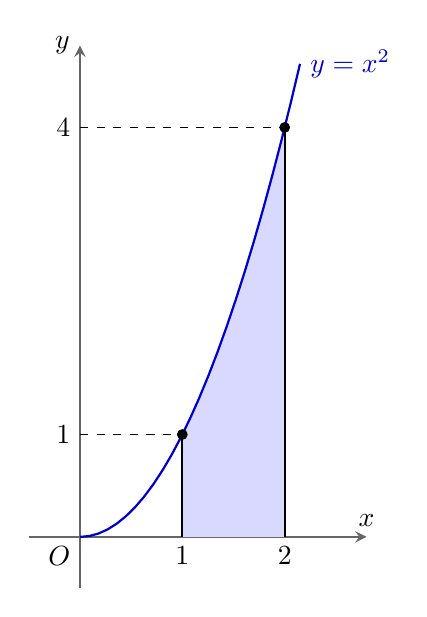
\begin{tikzpicture}[scale=1.3, >=stealth]
            % Axes
            \draw[->, gray!80!black, thick] (-0.5,0) -- (2.8,0) node[above, black] {$x$};
            \draw[->, gray!80!black, thick] (0,-0.5) -- (0,4.8) node[left, black] {$y$};
            \node[below left] at (0,0) {$O$};
            
            % Shaded area under y=x^2 from x=1 to x=2
            \fill[blue!15!white] (1,0) -- plot[domain=1:2] (\x, {\x*\x}) -- (2,0) -- cycle;
            
            % Plot y=x^2
            \draw[thick, blue!80!black, domain=0:2.15] plot (\x, {\x*\x}) node[right] {$y=x^2$};
            
            % Vertical lines
            \draw[thick] (1,0) -- (1,1);
            \draw[thick] (2,0) -- (2,4);
            
            % Dashed projection lines
            \draw[dashed] (0,1) -- (1,1);
            \draw[dashed] (0,4) -- (2,4);
            
            % Labels
            \fill (1,1) circle (1.5pt);
            \fill (2,4) circle (1.5pt);
            \node[below] at (1,0) {$1$};
            \node[below] at (2,0) {$2$};
            \node[left] at (0,1) {$1$};
            \node[left] at (0,4) {$4$};
        \end{tikzpicture}
        \par\vspace{0.5em} a)
    \end{minipage}
    \hfill
    \begin{minipage}{0.48\textwidth}
        \centering
        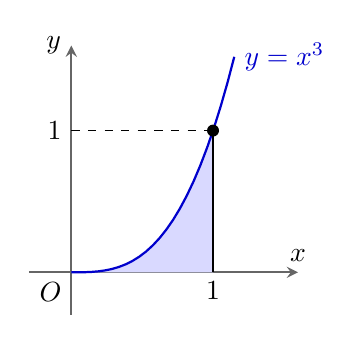
\begin{tikzpicture}[scale=1.8, >=stealth]
            % Axes
            \draw[->, gray!80!black, thick] (-0.3,0) -- (1.6,0) node[above, black] {$x$};
            \draw[->, gray!80!black, thick] (0,-0.3) -- (0,1.6) node[left, black] {$y$};
            \node[below left] at (0,0) {$O$};
            
            % Shaded area under y=x^3 from x=0 to x=1
            \fill[blue!15!white] (0,0) -- plot[domain=0:1] (\x, {\x*\x*\x}) -- (1,0) -- cycle;
            
            % Plot y=x^3
            \draw[thick, blue!80!black, domain=0:1.15] plot (\x, {\x*\x*\x}) node[right] {$y=x^3$};
            
            % Vertical line at x=1
            \draw[thick] (1,0) -- (1,1);
            
            % Dashed projection lines
            \draw[dashed] (0,1) -- (1,1);
            
            % Labels
            \fill (1,1) circle (1.2pt);
            \node[below] at (1,0) {$1$};
            \node[left] at (0,1) {$1$};
        \end{tikzpicture}
        \par\vspace{0.5em} b)
    \end{minipage}
\end{center}
\vspace{1.5em}
\noindent Tổng quát, ta có:

\begin{tcolorbox}[
    colback=blue!5!white,
    colframe=blue!75!black,
    sharp corners,
    boxrule=0pt,
    leftrule=3pt,
    top=8pt,
    bottom=8pt,
    left=12pt
]
    \textbf{\color{blue!80!black}Định lí 1:}
    \par\vspace{0.4em}
    Nếu hàm số $f(x)$ liên tục và không âm trên đoạn $[a; b]$, thì diện tích $S$ của hình thang cong giới hạn bởi đồ thị $y = f(x)$, trục hoành và hai đường thẳng $x = a$, $x = b$ là $S = F(b) - F(a)$, trong đó $F(x)$ là một nguyên hàm của hàm số $f(x)$ trên đoạn $[a; b]$.
\end{tcolorbox}

\begin{center}
    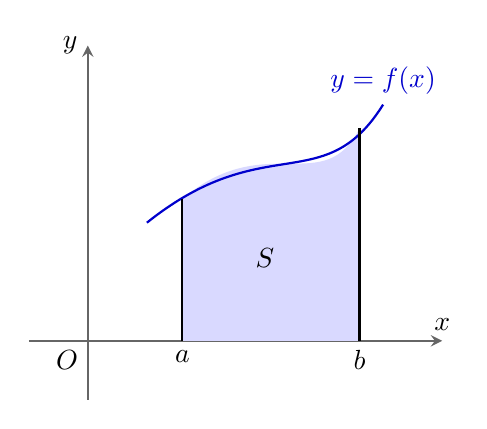
\begin{tikzpicture}[scale=1.5, >=stealth]
        % Axes
        \draw[->, gray!80!black, thick] (-0.5,0) -- (3.0,0) node[above, black] {$x$};
        \draw[->, gray!80!black, thick] (0,-0.5) -- (0,2.5) node[left, black] {$y$};
        \node[below left] at (0,0) {$O$};
        
        % Bounded area
        \fill[blue!15!white] (0.8,0) -- (0.8,1.2) .. controls (1.5,1.8) and (2.0,1.2) .. (2.3,1.8) -- (2.3,0) -- cycle;
        
        % Plot y=f(x)
        \draw[thick, blue!80!black] (0.5,1.0) .. controls (1.5,1.8) and (2.0,1.2) .. (2.5,2.0) node[above] {$y=f(x)$};
        
        % Vertical lines
        \draw[thick] (0.8,0) -- (0.8,1.2);
        \draw[thick] (2.3,0) -- (2.3,1.8);
        
        % Labels
        \node[below] at (0.8,0) {$a$};
        \node[below] at (2.3,0) {$b$};
        \node at (1.5,0.7) {$S$};
    \end{tikzpicture}
\end{center}

\vspace{1.5em}

\subsection*{\color{blue!80!black}b) Định nghĩa tích phân}

\begin{tcolorbox}[
    colback=blue!5!white,
    colframe=blue!75!black,
    sharp corners,
    boxrule=0pt,
    leftrule=3pt,
    top=8pt,
    bottom=8pt,
    left=12pt
]
    Cho $f(x)$ là hàm số liên tục trên đoạn $[a; b]$. Nếu $F(x)$ là một nguyên hàm của hàm số $f(x)$ trên đoạn $[a; b]$ thì hiệu số $F(b) - F(a)$ được gọi là \textbf{tích phân} từ $a$ đến $b$ của hàm số $f(x)$, kí hiệu là:
    \[
    \int_a^b f(x)dx
    \]
\end{tcolorbox}

\vspace{1em}
\noindent $\blacktriangleright$ \textbf{Chú ý:}
\begin{center}
    \begin{minipage}{\textwidth}
        \begin{enumerate}[label=\alph*), leftmargin=*, itemsep=0.8em]
            \item Hiệu $F(b) - F(a)$ thường được kí hiệu là $F(x)\big|_a^b$. Như vậy:
            \[
            \int_a^b f(x)dx = F(x)\Big|_a^b = F(b) - F(a)
            \]
            \item Ta gọi $\displaystyle \int_a^b$ là dấu tích phân, $a$ là cận dưới, $b$ là cận trên, $f(x)dx$ là biểu thức dưới dấu tích phân và $f(x)$ là hàm số dưới dấu tích phân.
            \item Trong trường hợp $a = b$ hoặc $a > b$, ta quy ước:
            \[
            \int_a^a f(x)dx = 0; \quad \int_a^b f(x)dx = -\int_b^a f(x)dx
            \]
        \end{enumerate}
    \end{minipage}
\end{center}

\vspace{1.5em}
\noindent $\blacktriangleright$ \textbf{Ý nghĩa hình học của tích phân:}
\par Nếu hàm số $f(x)$ liên tục và không âm trên đoạn $[a; b]$, thì tích phân $\displaystyle \int_a^b f(x)dx$ là diện tích $S$ của hình thang cong giới hạn bởi đồ thị $y = f(x)$, trục hoành và hai đường thẳng $x = a, x = b$. Vậy:
\[
S = \int_a^b f(x)dx
\]

\vspace{2.5em}

\section*{\color{blue!80!black}2. TÍNH CHẤT CỦA TÍCH PHÂN}

\noindent Cho $f(x), g(x)$ là các hàm số liên tục trên đoạn $[a; b]$. Khi đó, ta có:
\begin{enumerate}[label=\arabic*), leftmargin=*, itemsep=0.8em]
    \item $\displaystyle \int_a^b kf(x)dx = k\int_a^b f(x)dx \quad (k \text{ là hằng số})$;
    \item $\displaystyle \int_a^b [f(x) + g(x)]dx = \int_a^b f(x)dx + \int_a^b g(x)dx$;
    \item $\displaystyle \int_a^b [f(x) - g(x)]dx = \int_a^b f(x)dx - \int_a^b g(x)dx$;
    \item $\displaystyle \int_a^b f(x)dx = \int_a^c f(x)dx + \int_c^b f(x)dx \quad (a < c < b)$.
\end{enumerate}
\end{document}